\section{中断处理}

\begin{frame}
    \frametitle{中断处理现状观察}

    \begin{itemize}
        \item 参赛作品普遍不处理外部中断,仅处理时钟中断。
    \end{itemize}

    \begin{table}
        \centering
        \begin{tabular}{|c|c|}
            \hline \textbf{比赛队伍}               & \textbf{外部中断处理情况} \\
            \hline 清华大学 - ArceOS (Rust)        & 不处理               \\
            \hline 哈尔滨工业大学(深圳) - FTL OS (Rust) & 不处理               \\
            \hline 清华大学 - Maturin (Rust)       & 不处理               \\
            \hline 北京航空航天大学 - 图漏图森破 (C)        & 仅处理串口             \\
            \hline 西北工业大学 - NPUCore (Rust)     & 不处理               \\
            \hline MIT - xv6-riscv             & 处理串口和 virtio      \\
            \hline
        \end{tabular}
    \end{table}


\end{frame}

\begin{frame}
    \frametitle{原因分析}

    \begin{enumerate}
        \item 客观原因
              \begin{itemize}
                  \item 硬件厂商不愿意公开手册
                  \item SoC 上中断处理部件标准不统一
              \end{itemize}
        \item 比赛原因
              \begin{itemize}
                  \item RISC-V SBI 提供了 debug console 可用于串口 IO
                  \item 比赛对外设没有要求
              \end{itemize}
        \item 教学原因
              \begin{itemize}
                  \item 组成原理课程缺少对 CPU 核外 SoC 上部件的讲解
              \end{itemize}
    \end{enumerate}


\end{frame}


\begin{frame}
    \frametitle{中断处理实现}

    \begin{itemize}
        \item MankorOS 根据 RISC-V PLIC 标准实现了中断处理
    \end{itemize}

    \begin{figure}
        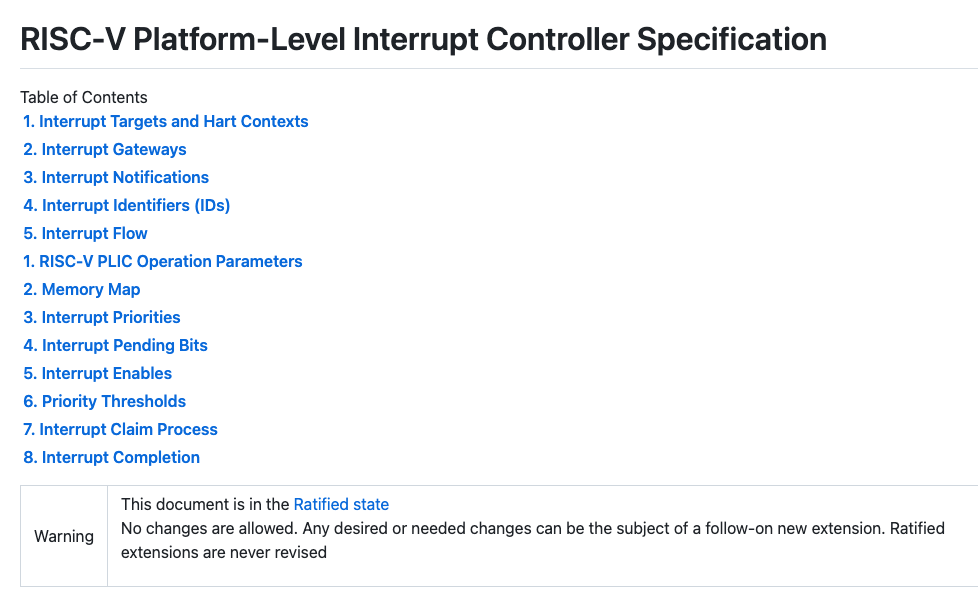
\includegraphics[width=.5\textwidth]{assets/plic.png}
    \end{figure}

\end{frame}